\subsection{Introduction}

Often, the desired goal is to reduce the dimensions of a N-dimensional dataset by projecting it onto a k-dimensional subspace (where k\textless N) in order to increase the computational efficiency while retaining most of the information.

A summary of the Principal Component Analysis is the following:
\begin{enumerate}
    \item Standarise the data
    \item Obtain the covariance matrix
    \item Obtain the \emph{eigenvectors} and their correspondent \emph{eigenvalues}
    \item Sort the eigenvalues in descending order of magnitude to chose the \emph{k} eigenvectors that correspond to the \emph{k} largest eigenvalues
    \item Construct the projection matrix \emph{\textbf{W}} from the selected \emph{k} eigenvectors
    \item Transform the original dataset \emph{\textbf{X}} via \emph{\textbf{W}} to obtain a k-dimensional feature subspace \emph{\textbf{Y}}
\end{enumerate}

\subsection{Standarisation}
All variables must be on the same scale with a \texttt{standard scaler}:

$$
x_d = \frac{x_d - \overline{x}_d}{\sqrt{
\sum \frac{(x_d - \overline{x}_d)^2}{N}}}
$$

Here is the code:
\begin{lstlisting}[language=Python]
import numpy as np

# 0. Define data
X = np.random.rand(200,10)

# Make X not to be in scale 0-1
d = np.random.poisson(20,10)
X = np.multiply(X,d)

def standarisation(X):
    for d in range(X.shape[1]):
        X[:,d] = (X[:,d] - X[:,d].mean()) / X[:,d].std()
    return X

# 1. Standarise data
X_std = standarisation(X.copy())
\end{lstlisting}

\subsection{Covariance matrix, Eigenvalues, and Eigenvectors}
The classic approach to PCA is to perform the eigendecomposition on the covariance matrix $\Sigma$, which is a $d \cdot d$ matrix where each element represents the covariance between two variables, calculated as follows:

$$
\sigma_{j,k} = \frac{1}{n-1}\sum_{i=1}^N {(x_{i,j} - \overline{x}_{j})} \cdot {(x_{i,k} - \overline{x}_{k})}
$$

With some algebra, this equation can be summarised into:
$$
\Sigma = \frac{1}{n-1}\sum_{i=1}^N {(X - \overline{x})^T}{(X - \overline{x})}
$$

In Python code:

\begin{lstlisting}[language=Python]
# Get mean
mean_vec = np.mean(X_std, axis=0)

# 2. Get covariance matrix
cov_mat = (X_std - mean_vec).T.dot((X_std - mean_vec)) / (X_std.shape[0]-1)
\end{lstlisting}

Next, eigenvalues and the eigenvectors are obtained:

\begin{lstlisting}[language=Python]
# 3. Eigen decomposition
eig_vals, eig_vecs = np.linalg.eig(cov_mat)
\end{lstlisting}

Sometimes, they are calculated with the correlation matrix \textbf{\emph{X}}. Nevertheless, this method yields the same results since the correlation matrix can be understood as the normalized covariance matrix. This statement is tested here:

\begin{lstlisting}[language=Python]
# 3. Eigendecomposition
cov_mat = np.cov(X_std.T)
eig_vals, eig_vecs = np.linalg.eig(cov_mat)
print(eig_vals)

[Out]:[ 1.43557072  0.62102126  0.77387224  0.79279969  1.20947608  1.15829268
  0.93869466  0.99929095  1.07098582  1.05024716]

# 4. Test cor_mat
cor_mat1 = np.corrcoef(X_std.T)
eig_vals_, eig_vecs_ = np.linalg.eig(cor_mat1)
print(eig_vals_)

[Out]: [ 1.42839287  0.61791616  0.77000288  0.78883569  1.2034287   1.15250122
  0.93400118  0.99429449  1.06563089  1.04499592]

\end{lstlisting}

\subsection{Sort eigenvalues}
Which eigenvector(s) can dropped without losing too much information? Eigenvectors with the lowest eigenvalues bear the least information about the distribution of the data and, therefore, they can be dropped.

The eigenvalues are ranked to choose the top \emph{k} eigenvectors:

\begin{lstlisting}[language=Python]
# 5. Sort eigenvalues
eig_pairs = [(np.abs(eig_vals[i]), eig_vecs[:,i]) for i in range(len(eig_vals))]
eig_pairs.sort()
eig_pairs.reverse()
\end{lstlisting}

\subsection{Explained variance}

How many principal componets we choose for the new feature space? A useful measure is the \emph{explained variance}. The explained variance is calculated from the eigenvalues and tells us how much information or variance can be attributed to each of the principal components. It can be calculated and plotted as follows:

\begin{lstlisting}[language=Python]
import matplotlib.pyplot as plt
import datetime
import os
fig, ax1 = plt.subplots()
components = range(len(var_exp))
color = 'deeppink'
ax1.set_xlabel('Components')
ax1.set_ylabel('Explained Variance', color=color)
ax1.bar(components, var_exp, color=color)
ax1.tick_params(axis='y', labelcolor=color)

ax2 = ax1.twinx()  # instantiate a second axes that shares the same x-axis
color = 'blue'
ax2.set_ylabel('Cumulative Explained Variance', color=color)
ax2.errorbar(components, cum_var_exp, marker='o', color=color, ls='dotted')
ax2.tick_params(axis='y', labelcolor=color)
plt.xlabel('Components')
plt.xticks(list(components))
fig.tight_layout()
dirpath = '/Users/dnarganes/PhD/PCA_raw/pics'
if not os.path.exists(dirpath):
    os.makedirs(dirpath)
filename = 'img_{}.png'.format(datetime.datetime.now())
plt.savefig(os.path.join(dirpath,filename))
\end{lstlisting}

\begin{figure}[H]
\centering
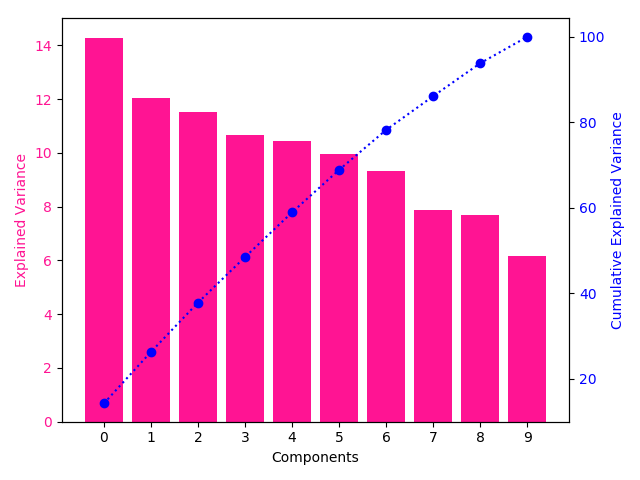
\includegraphics[width=12cm]{pics/pca_var_exp.png}
\end{figure}

The above plot shows that the first three components account for the 0.3 of the variance. Take into account that the defined matrix \emph{\textbf{X}} was defined as from a normal random distribution. With a real dataset I could take the first \emph{k} components that account for most of the variance.

\subsection{Y and W matrices}
The aim is to reduce the \emph{d} dimensional feature space to a 2 dimensional feature subspace by choosing the top 2 eigenvectors to make the reduced eigenvector matrix \emph{\textbf{W}}. Finally, the dot product of \emph{\textbf{X}} and \emph{\textbf{W}} matrices gives me the \emph{\textbf{Y}} matrix.

\begin{lstlisting}[language=Python]
# 6. Projection onto new feature subspace
matrix_w = np.hstack((eig_pairs[0][1].reshape(len(components),1), 
                      eig_pairs[1][1].reshape(len(components),1)))

Y = X_std.dot(matrix_w)
print(Y.shape)

[Out]: (200,2)
\end{lstlisting}

